% Chapter Template

\chapter{Caso d'uso: fine-tuning su dataset arbitrario} % Main c
\label{Capitolo6} % Change X to a consecutive number; for referencing this chapter elsewhere, use \ref{ChapterX}
\def \path {Figures/C6}
Un tipico scenario d'uso industriale è quello di avere un piccolo dataset di immagini annotate a disposizione e, da questo, dover costruire un modello che riesca a generalizzare bene su esempi ancora mai visti. In questo capitolo si vedrà come affrontare questo problema utilizzando le convolutional neural networks ed il \emph{transfer learning}.
%--------------------------------------------------------------------
%	SECTION 1
%--------------------------------------------------------------------
\section{Il problema}
Occorre trovare una maniera di costruire un modello che riesca ad essere addestrato su un dataset discretamente piccolo ma al contempo sia successivamente capace di classificare correttamente esempi ancora non visti. Le CNN sono la norma quando si tratta di task di classificazione, tuttavia è difficile riuscire ad affrontare un problema del genere per i seguenti motivi: 
\begin{enumerate}
\item un modello troppo semplice non sarebbe capace di estrarre tutte le caratteristiche necessarie per catalogare le immagini; 
\item addestrare finemente un modello complesso richiede delle risorse computazionali non indifferenti, non a disposizione;
\item un modello troppo complesso con un dataset troppo piccolo avrebbe la certezza di incorrere in overfitting.
\end{enumerate}
\\
In pratica, in pochi addestrano interamente una CNN da zero proprio per i problemi elencati sopra. Quello che in genere si fa è usare modelli pre-addestrati per settimane su un dataset enorme come quello di \emph{Imagenet\href{http://www.image-net.org/}} come estrattori di features da applicare a dataset più piccoli per i più svariati scopi.


%--------------------------------------------------------------------
%	SECTION 2
%--------------------------------------------------------------------
\section{Transfer Learning}
Sfruttare l'apprendimento di grosse CNN per trasferirlo alla nostra rete è un processo che prende il nome di \emph{"transfer learning"}. \\
Gli scenari principali del transfer learning sono i seguenti: 
\begin{itemize}	
\item \textbf{CNN come estrattore di feature}: si prende una rete addestrata su ImageNet, si rimuove l'ultimo strato completamente connesso che faceva da classificatore per le 1000 classi di ImageNet, e si utilizza la restante rete come estrattore di features per il nuovo dataset. Si danno in ingresso alla rete le immagini del nuovo dataset e si ottengono in uscita le attivazione dell'ultimo hidden layer prima del classificatore finale, chiamate anche \emph{CNN codes}. Una volta ottenuti questi CNN codes, gli si addestra un classificatore lineare (una SVM o un SoftMax).
\\
Uno schema di questo approccio si è visto nella figura \ref{fig:cnn1} del Capitolo \ref{Capitolo3}, dove il primo rettangolo rossa indica la CNN come estrattore di features. 
\item \textbf{Fine-tuning su una CNN}: la seconda strategia consiste non solo nel rimpiazzare e ri-addestrare il classificatore usando CNN sul nuovo dataset; ma anche nel "rifinire" (fine-tune) i pesi di tutta la CNN continuando la backpropagation. Si possono rifinire i pesi di tutti gli strati o solamente dei primi se si hanno preoccupazioni di overfitting. Questa scelta è motivata dal fatto che i primi strati della rete contengono feature più generiche (per esempio edge detectors) che possono essere utili a diversi task, mentre gli ultimi strati diventano sempre più specifici ai dettagli delle classi contenuti nel dataset su cui sono state addestrate. Ad esempio, una CNN addestrata sull'ImageNet challenge che contiene tantissime razze diverse di cane, può avere molto del suo potere di rappresentazione dedito a distinguire tra le diverse razze. 
\end{itemize} \\
Siccome le archittuture moderne richiedono un addestramento di 2-3 settimane su una moltitudine di GPUs, nella comunità scientifica è consueto rilasciare la rete addestrata on-line, cosicché gli altri ne possano beneficiare. Ad esempio, il framework per il Deep Learning \emph{"Caffe"} ha una repository online chiamato "Model Zoo"\parencite{Wzoo}, dove appunto gli utenti caricano i pesi sinaptici dei loro modelli già addestrati. Grazie a delle librerie che traducono le rappresentazioni dei modelli da un framework ad un altro, è facile importare questi modelli (in Torch, ad esempio).   

\subsection{Fine-tuning}
Il fine-tuning è il processo con il quale si rifiniscono i pesi della rete alle specificità del dataset su cui la si sta addestrando. Come visto prima, è una strategia molto vantaggiosa poiché è un risparmio sia in termini di sviluppo di software ma soprattutto in termini di risorse computazionali. 

Tuttavia, vi sono dei rischi nel fine-tuning che si possono arginare ricorrendo ad alcune buone pratiche che fanno riferimento soprattutto a 2 fattori: \emph{la dimensione} del nuovo dataset e \emph{la similarità} al dataset su cui la rete è stata pre-addestrata. \\
A questo proposito le combinazioni possibili sono 4: 
\begin{enumerate}
\item \emph{Il nuovo dataset è piccolo e simile al dataset originale}:  poiché ci sono pochi dati, non è una buona idea fare il fine-tuning dell'intera rete a causa dell'overfitting. Siccome il dataset è simile all'originale ci si può aspettare che le anche le features degli ultimi livelli della CNN siano rilevanti per questi dati. Di conseguenza, la miglior idea è addestrare un classificatore lineare sui CNN Codes.

\item \emph{Il nuovo dataset è grande e simile al dataset originale}: dal momento che si hanno molti dati a disposizione, si ha più confidenza che la rete non presenti overfitting se si esegue il fine-tuning su tutti gli strati.

\item \emph{Il nuovo dataset è piccolo ma molto diverso dal dataset originale}: siccome i dati sono pochi, probabilmente la scelta migliore è addestrare un classificatore lineare. E siccome il dataset è  molto diverso, non conviene addestrarlo sull'ultimo layer della CNN; è meglio addestrarlo sulle attivazioni di uno degli strati precedenti. 
\item \emph{Il nuovo dataset è grande e molto piccolo dal dataset originale}: dato che è il dataset è grande è possibile addestrare una CNN da zero. In pratica però, è sempre vantaggioso inizializzare i pesi da un modello pre-addestrato rispetto ad una inizializzazione random. Dopodiché, ci si può aspettare che un fine-tuning totale della rete funzioni avendo a disposizioni tanti dati. 
\end{enumerate}
\\
\\
Un ultimo punto a tenere a mente riguarda il \emph{learning rate}: è caldamente consigliato usare learning rate più bassi del solito quando si esegue il fine-tuning. Questo perché si parte dal presupposto che i pesi siano già regolati relativamente bene e non si vuole distorcerli troppo o troppo velocemente, a maggior ragione se sopra questi avviene l'addestramento di un classificatore lineare i cui pesi invece vengono inizializzati in maniera casuale.  
\section{Dataset}
Il dataset d'esempio contiene 377 immagini appartenenti a 2 classi: api e formiche. Il training set è costituito da 224 immagini, mentre 153 sono per il validation set. Si noti a questo punto, la differenza di 2 ordini di grandezza rispetto ai dataset usato nel Capitolo \ref{Capitolo4}, che contenevano 60 mila immagini ciascuno; e la differenza di 4 ordini di grandezza con ImageNet su cui è stata pre-addestrata ResNet. \\
Alcuni esempi delle immagini nel dataset si possono osservare nelle figure \ref{fig:bee} e \ref{fig:ant}. 
\begin{figure}[h!]
 \centering
 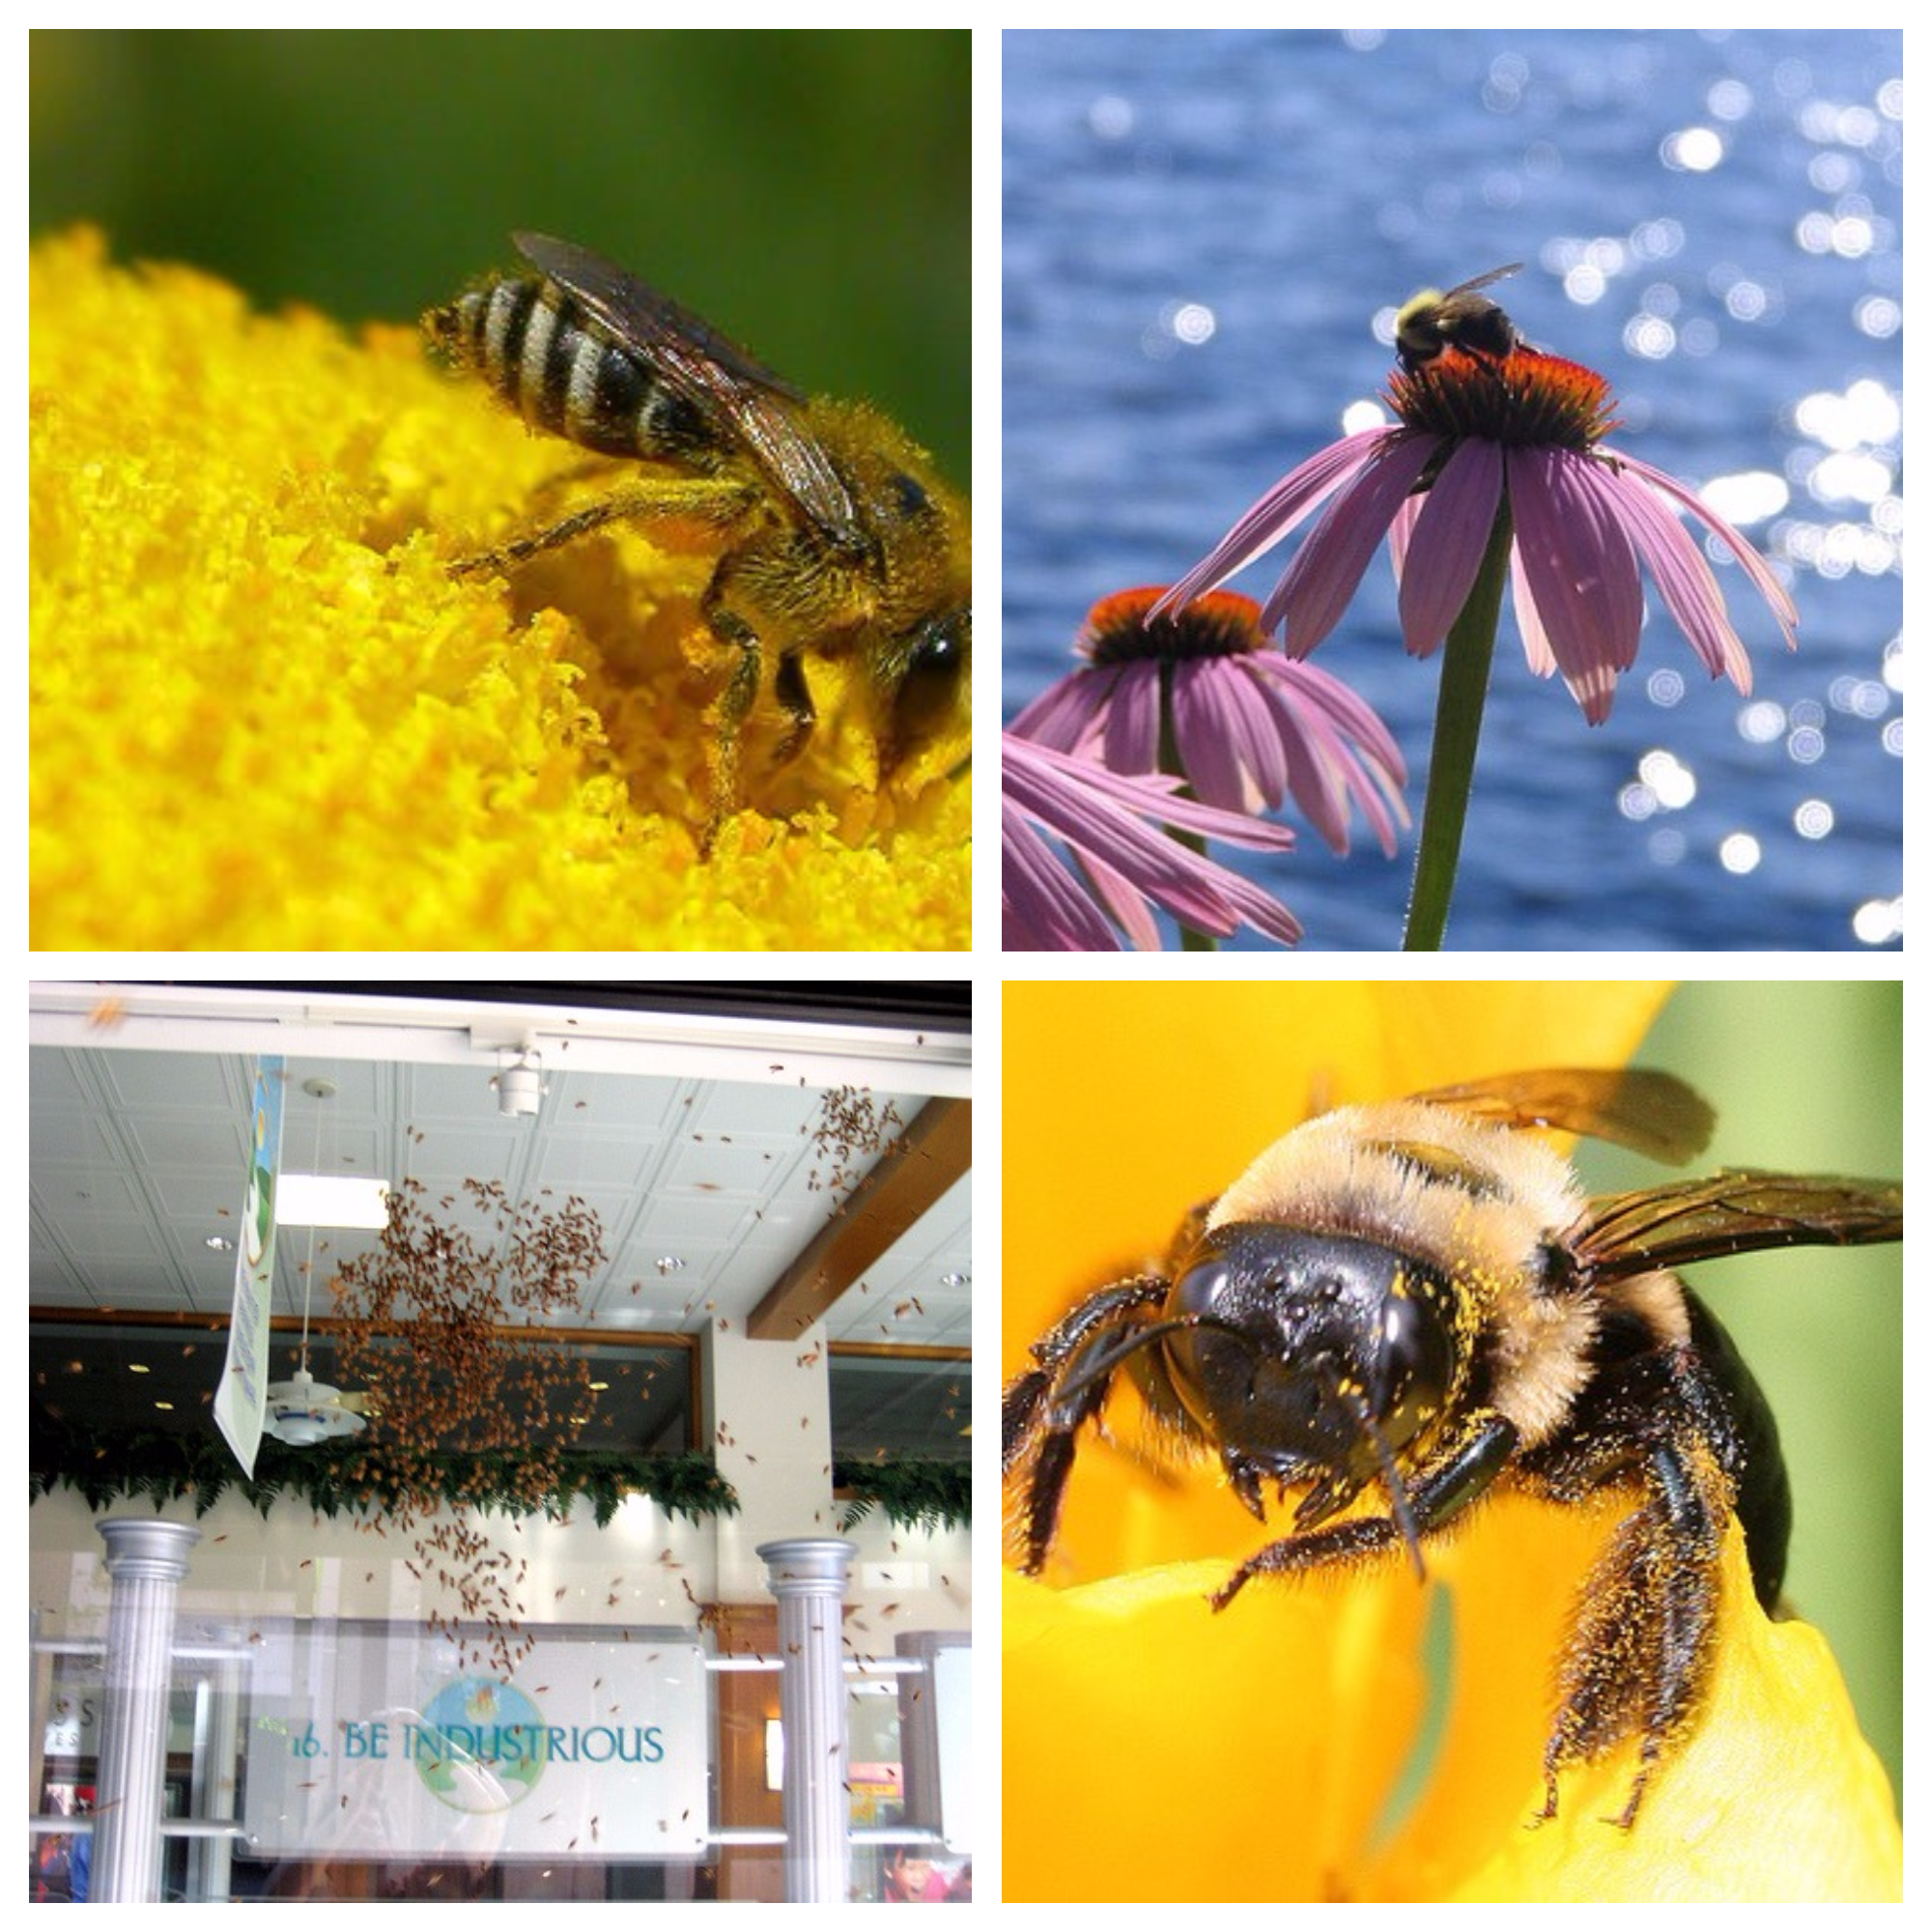
\includegraphics[width=0.6\textwidth]{\path/bee-collage.png} 
 \caption{Alcuni esempi delle immagini delle api del dataset}
 \label{fig:bee}
\end{figure}
\begin{figure}[h!]
 \centering
 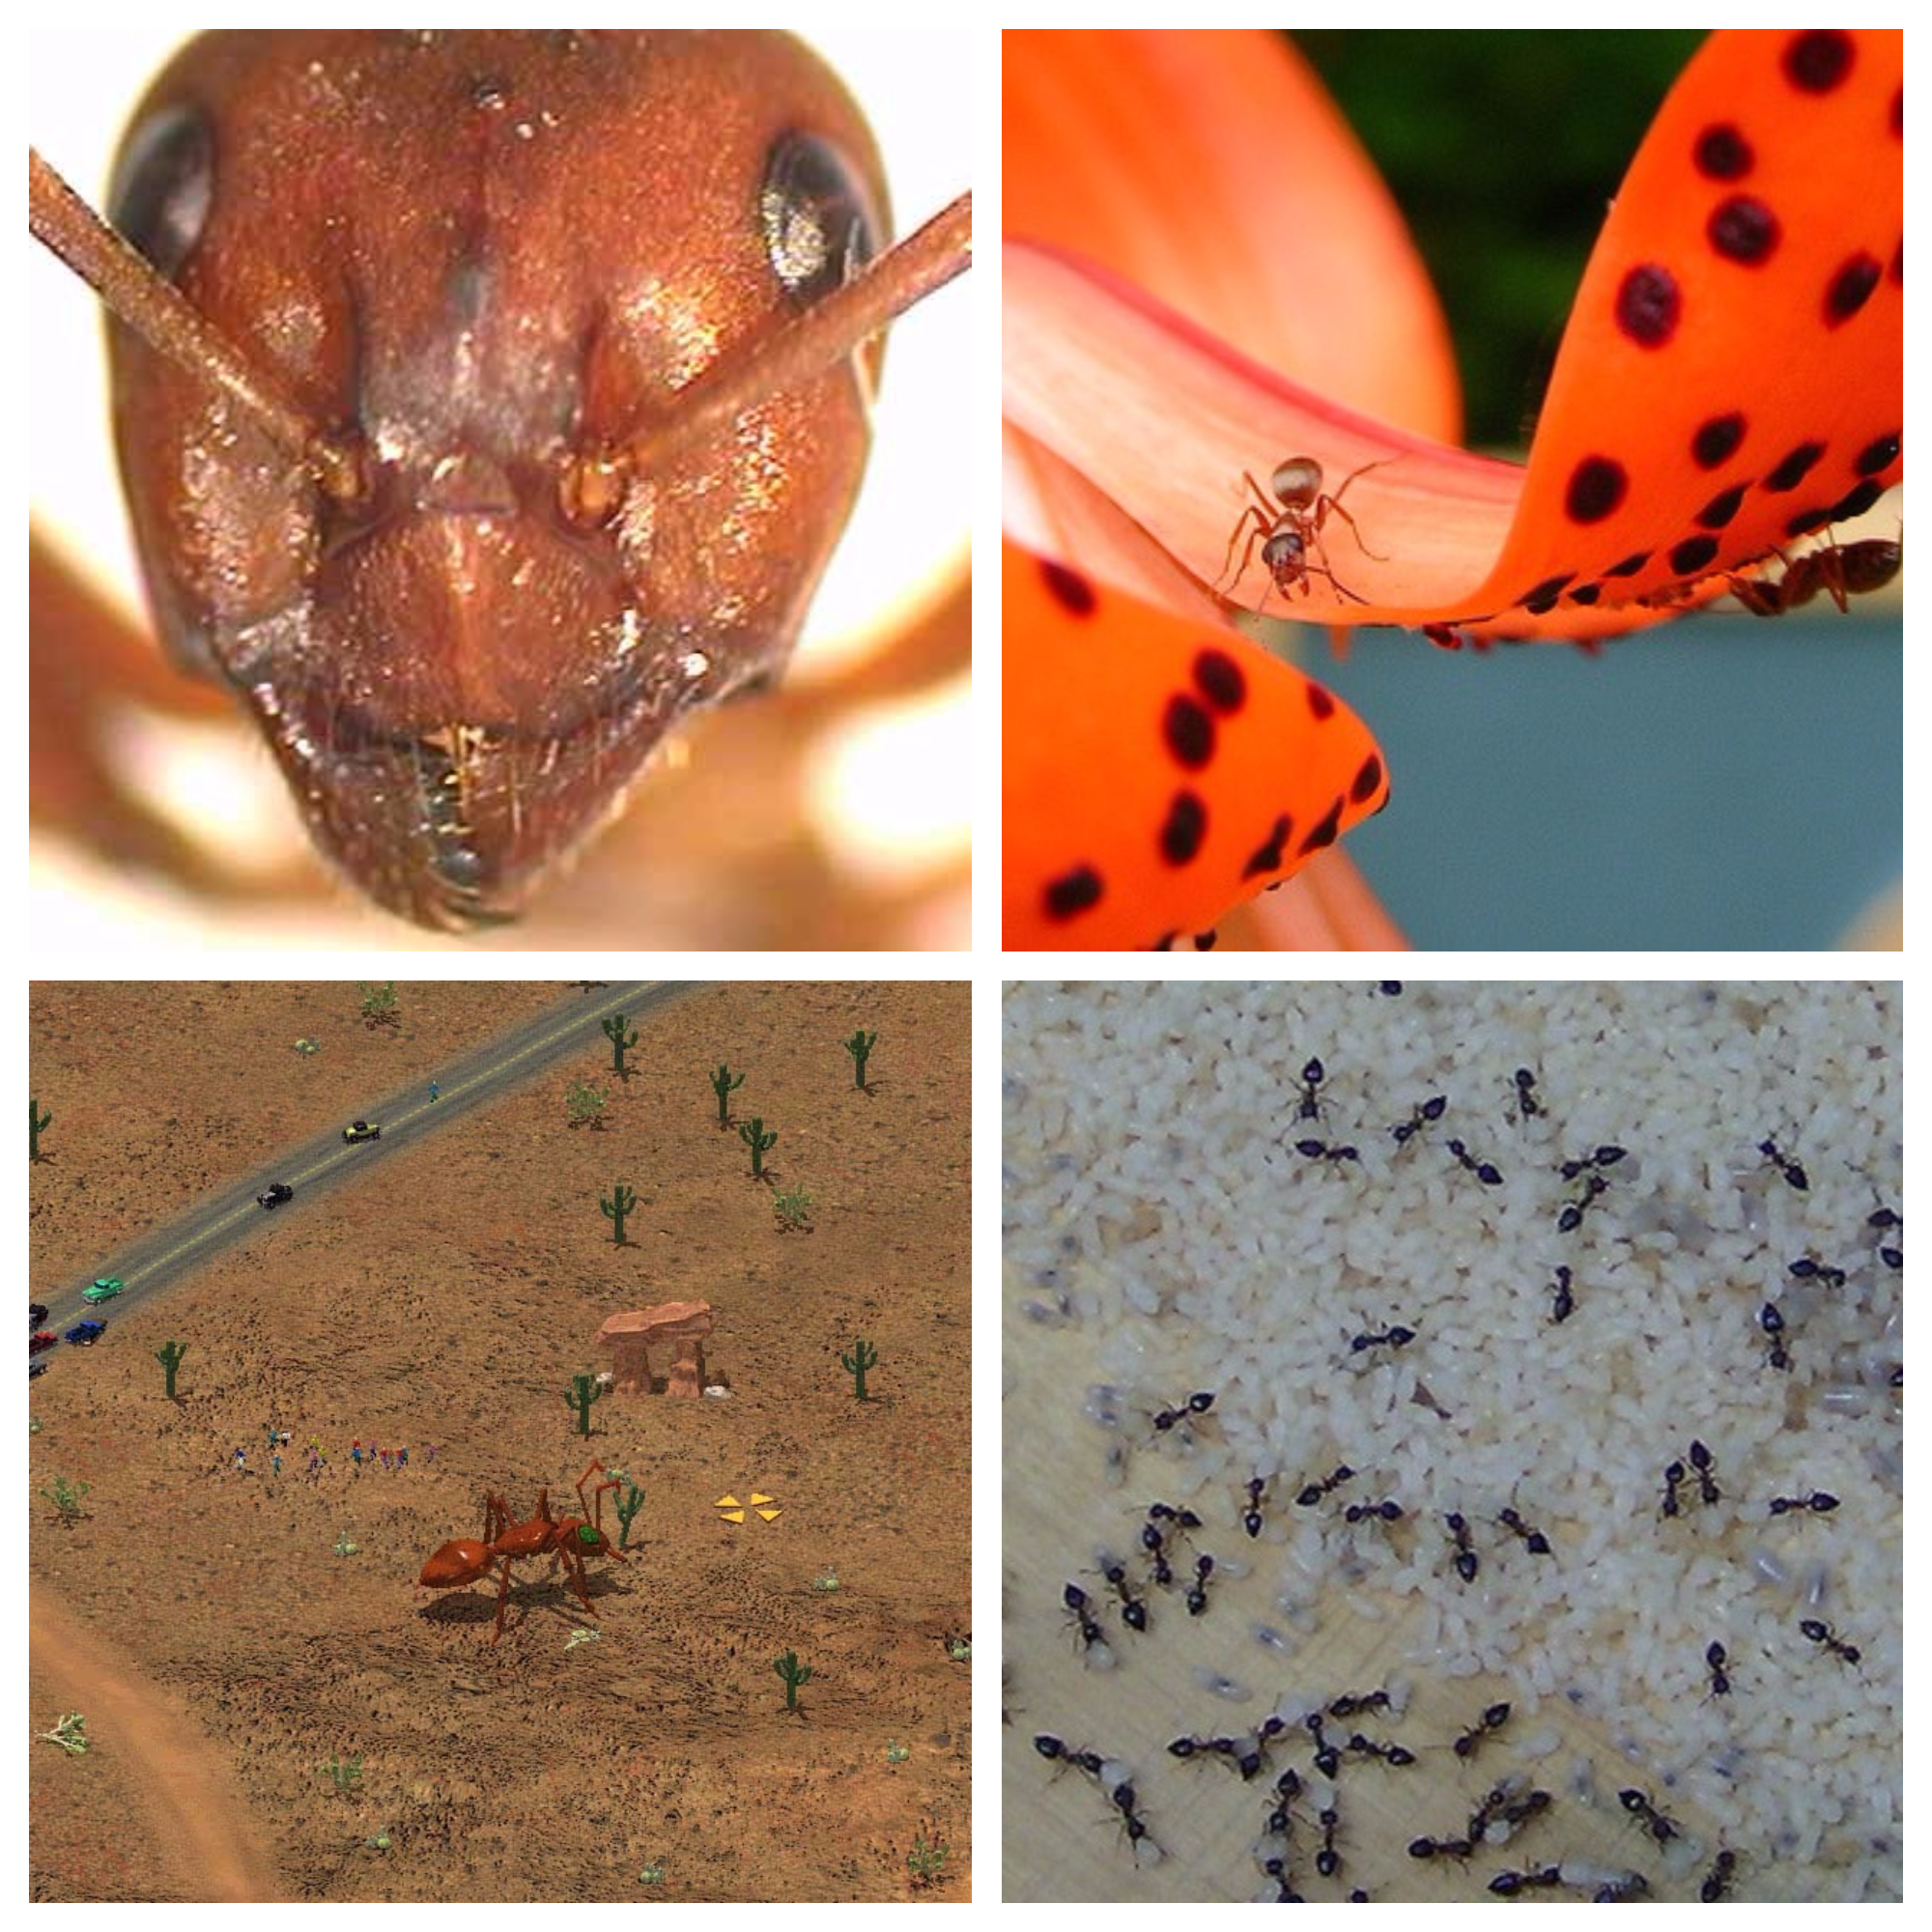
\includegraphics[width=0.6\textwidth]{\path/ant-collage.png} 
 \caption{Alcuni esempi delle immagini delle formiche del dataset}
 \label{fig:ant}
\end{figure}

Utilizzando un modello pre-addestrato si estraggono i CNN Codes, ovvero le feature che si hanno in output dagli ultimi layer di convoluzione e si salvano in due file \texttt{'train\_ants.t7'} e \texttt{'train\_bees.t7'} (t7 è il formato specifico usato da Torch). Dopodiché, si caricano i dati nei tensori, gli si associano le label corrette (1 e 2) e li si prepara per il training. 


\begin{lstlisting}[language={[5.2]Lua}]
--Load features for training
t1 = torch.load(opt.data..'train_ants.t7').features:float()
t2 = torch.load(opt.data..'train_bees.t7').features:float()
Z = torch.cat(t1, t2, 1) --CNN Codes
dataDim = Z:size(2)

--1: ants
--2: bees
classes = {1,2}
lab1 = torch.Tensor(t1:size(1)):fill(1)
lab2 = torch.Tensor(t2:size(1)):fill(2)
labels = torch.cat(lab1, lab2)

--Shuffling the whole given dataset before dividing it in training and val sets
torch.manualSeed(opt.manualSeed)
shuffle= torch.randperm(Z:size(1))

--Creating the datasets objects for the validation and training sets

validationset={}
-- we are going to use 30 % of the whole dataset as the validation set
-- the ratio can be changed using the validationSize option
function validationset:size() return opt.validationSize * Z:size(1) end
for i=1, validationset:size() do
   validationset[i]={Z[shuffle[i]], labels[shuffle[i]]}
end

trainingset={}
function trainingset:size() return Z:size(1) - validationset:size() end
for i=1, trainingset:size() do
   trainingset[i]={Z[shuffle[ validationset:size()+ i ]], labels[shuffle[ validationset:size()+i ]]}
end
\end{lstlisting}



%--------------------------------------------------------------------
%	SECTION 3
%--------------------------------------------------------------------
\section{Fine-tuning su Resnet}
\subsection{Training}
Come menzionato nel Capitolo 5, Facebook ha reso pubbliche le sue implementazioni di ResNet, compresi i pesi dei modelli pre-addestrati su ImageNet (1.2 millioni di esempi). È stato utilizzato il modello da 18 strati, sopra il quale si è addestrato un classificatore SoftMax. La funzione SoftMax\parencite{WSoftmax} generalizza la funzione logistica con una funzione esponenziale normalizzata: 
$$
\sigma(z) = \frac{e^{z_j}}{\sum_{K}^{k=1}e^{z_k}} \quad per \quad j=1,..., K.
$$
\\
L'architettura finale è raffigurata in \ref{fig:arch}. 
\begin{figure}[h!]
 \centering
 \includegraphics[width=1.0\textwidth]{\path/ft-arch.png} 
 \caption{Architettura della rete: il transfer learning avviene utilizzando i CNN codes provenienti da ResNet per addestrare il classificatore SoftMax}
 \label{fig:arch}
\end{figure}
Per addestrare il classificatore lineare non è necessario ricorrere alla libreria di ottimizzazione \texttt{optim} di Torch usata per il training delle CNN. Basta utilizzare un modulo di training più semplice chiamato \texttt{StochasticGradient}, che appunto lo allenerà mediante una discesa del gradiente classica.
\\
Di default, questo modulo stampa sul terminale solo l'errore corrente. Tuttavia, per riuscire a capire se sta avvenendo overfitting o meno, bisogna definire una funzione di valutazione che verrà chiamata poi durante il training dalla funzione di callback del modulo di training.

\begin{lstlisting}[language={[5.2]Lua}]
--Defining the evaluation function
function eval(model, dataset, validation)
   local correct=-1
   local r={}
   for i=1, dataset:size() do
      local example=dataset[i]
      local img = example[1]
      local label = example[2]
      local prediction= model:forward(img) --this output the prob (class \| image)
      local confidences, indices = torch.sort(prediction, true) -- let's sort the prob
      r[i]=indices[1] -- Picking up the class with highest confidence
      if validation then --If this is the validation set we can estimate the accuracy
         if r[i]==label then
            correct=correct+1
         end
      end
   end
   return r, correct
end
\end{lstlisting}
\\
Una volta definita la funzione di valutazione, definiamo la callback function che avrà queste funzioni: 
\begin{itemize}
\item chiamerà la funzione di valutazione sul training e sul validation set; 
\item stamperà le rispettive percentuali di accuratezza; 
\item farà logging dei dati per un'eventuale plotting off-line degli stessi.
\end{itemize} 

\begin{lstlisting}[language={[5.2]Lua}]
local function evaluation_callback(trainer, iteration, currentError)
   _, correct=eval(trainer.module, trainingset, true)
   training_acc= correct / trainingset:size()
   print("# test accuracy = " .. training_acc)

   _, correct=eval(trainer.module, validationset, true)
   acc = correct / validationset:size()
   print("# validation accuracy = " .. acc)

   --save values to be logged later on
   if trainer.stats then
      logger:add{iteration, training_acc, acc}
      trainer.stats.tr[iteration]=training_acc
      trainer.stats.val[iteration]=acc
   end
end
\end{lstlisting}
\\
A questo punto possiamo lanciare l'addestramento.

\begin{lstlisting}[language={[5.2]Lua}]
--define the trainer parameters
trainer = nn.StochasticGradient(model, criterion)
trainer.hookIteration=evaluation_callback --link callback function
trainer.stats={tr={},val={}} --we will use this table to save the stats
trainer.learningRate = opt.LR
trainer.maxIteration = opt.nEpochs -- epochs of training
trainer.verbose = false -- print stats in the callback
--let's train
trainer:train(trainingset)
--save model
torch.save(opt.save..'tuned.t7', model)
\end{lstlisting}
\\
In output si ottiene qualcosa di simile a: 
\begin{lstlisting}	
# StochasticGradient: training
# .....	
# training accuracy = 0.84248771281362	
# validation accuracy = 0.72571834721429	
# current error = 1.89795655439887	
# training accuracy = 0.84428662170892	
# validation accuracy = 0.76952567752381
# .....	
\end{lstlisting}

\\
I risultati sono in figura \ref{fig:res-train}. Come si nota, l'addestramento è andato a buon fine e la rete non ha dato problemi di overfitting, quindi il classificatore è effettivamente pronto per distinguere le api dalle formiche. Nella sezione \ref{subsec:c6-testing} lo si mette alla prova. 
\begin{figure}[h!]
 \centering
 \includegraphics[width=1.0\textwidth]{\path/Figure1.png} 
 \caption{Curve di apprendimento sul nuovo dataset: il modello generalizza in maniera ottimale e non vi sono segni di overfitting}
 \label{fig:res-train}
\end{figure}

\subsection{Testing}
\label{subsec:c6-testing}
È il momento di testare il classificatore su esempi ancora non visti. In precedenza si sono salvati su altri due file le immagini di testing; si caricano queste immagini nei tensori, gli si associa le label corrette e si utilizza la stessa funzione di valutazione usata nel training per avere in uscita la categoria scelta dalla rete. Dopodiché si confronta questa risposta con la rispettiva label e si conta la percentuale di classificazioni corrette. 

\begin{lstlisting}[language={[5.2]Lua}]
--load model and save prediction on unseen test data
model = torch.load(opt.save..'tuned.t7')
t1 = torch.load(opt.data..'test_ants.t7').features
t2 = torch.load(opt.data..'test_bees.t7').features
Z = torch.cat(t1,t2,1)

labels = torch.Tensor(t1:size(1)):fill(1)
lab2 = torch.Tensor(t2:size(1)):fill(2)
labels = torch.cat(labels, lab2)

dataset={}
function dataset:size() return Z:size(1)  end

for i=1, dataset:size() do
    dataset[i]={Z[i]:float()}
end

pred,_ = eval(model, dataset, false)

output={}
correct = 0
for i=1,#pred do
  if labels[i] == pred[i] then
    correct = correct + 1
  end
  output[i]={id=i,Label=pred[i]}
end
accuracy = correct / labels:size(1)
print('Testing on '..labels:size(1)..' unseen examples...')
print(string.format('#Test Accuracy: %.3f',accuracy))
--save results in a CSV file
csvigo.save('test.csv', output, true)
\end{lstlisting}

Eseguendo il test si ottiene l'output in figura \ref{fig:res-test}. 
\begin{figure}[h!]
 \centering
 \includegraphics[width=1.0\textwidth]{\path/test-unseen-data.jpg} 
 \caption{Testing della rete su 154 esempi ancora non visti. Accuracy = 95.4\%}
 \label{fig:res-test}
\end{figure}
\\

Si è quindi dimostrato come addestrare con risultati eccellenti un classificatore su di un dataset arbitrario molto piccolo sfruttando una rete allo stato dell'arte. 

